 \documentclass[a4paper]{article}
\usepackage{multirow}
\usepackage{amsmath}
\usepackage{amssymb}
\usepackage{geometry}
\usepackage{amsthm}
\usepackage{mathtools}
\usepackage{graphicx}
\usepackage{nicematrix}
\usepackage{array}
\usepackage{subfig}
\graphicspath{ {./images/} }


\geometry{left=2.5cm,right=2.5cm,top=0cm,bottom=1.5cm}

\renewcommand\qedsymbol{$\blacksquare$}

\linespread{1.2}

\definecolor{lightgray}{gray}{0.5}

\title{Optimization II Homework 3 Solution}
\author{Lu Tuxun\\
	\ttfamily{tlu32@jhu.edu}}

\newcommand{\abs}[1]{\lvert #1 \rvert}

\begin{document}

	\maketitle
	\section*{Problem 1}
	\begin{verbatim}
	load('/Users/nicklu/JHU/2022Spring/Intro to Opt2/hw03/hw1_1.mat');

	thecolors = color(edgelist,2)
	\end{verbatim}

  \color{lightgray} \begin{verbatim}
	thecolors =

		     2
		     1
		     2
		     1
		     1
		     2
		     1
		     2

\end{verbatim} \color{black}

 \begin{verbatim}
load('/Users/nicklu/JHU/2022Spring/Intro to Opt2/hw03/hw1_2.mat');


thecolors = color(edgelist,3)
\end{verbatim}

        \color{lightgray} \begin{verbatim}
thecolors =

     3
     1
     2
     3
     1
     2
     3
     3
     2
\end{verbatim} \color{black}
    \begin{verbatim}
load('/Users/nicklu/JHU/2022Spring/Intro to Opt2/hw03/hw1_3.mat');


thecolors = color(edgelist,3)
\end{verbatim}
\newpage
\hspace{3cm}
        \color{lightgray} \begin{verbatim}
thecolors =

     3
     1
     3
     2
     1
     2
     3
     1
     1
     2

\end{verbatim} \color{black}
    
For the last graph, I get a 6-coloring in 2.841599 seconds and 5-coloring in 27.283567 seconds using GUROBI. 4-coloring seems, and indeed infeasible. I tried to run it on my computer, having 100\% CPU usage and it became super hot, but no result came out after 20 minutes.

	\section*{Problem 2}
	I affirm that I read and understand the solution for 2021 Exam1, Problem 5.

	\section*{Problem 3}

	Since paths and even cycles of half-present edges can be broken down, selecting alternating edges to be disjoint fully-present edges in the matching, with cardinality at least as great. The only way to make $\alpha'_f(G) > \alpha'(G)$ different is when there are odd cycles in a graph. In an odd cycle graph, $\alpha'_f(G)=\alpha'(G)+\frac{1}{2}$:
	\begin{figure}[h]
        \centering
        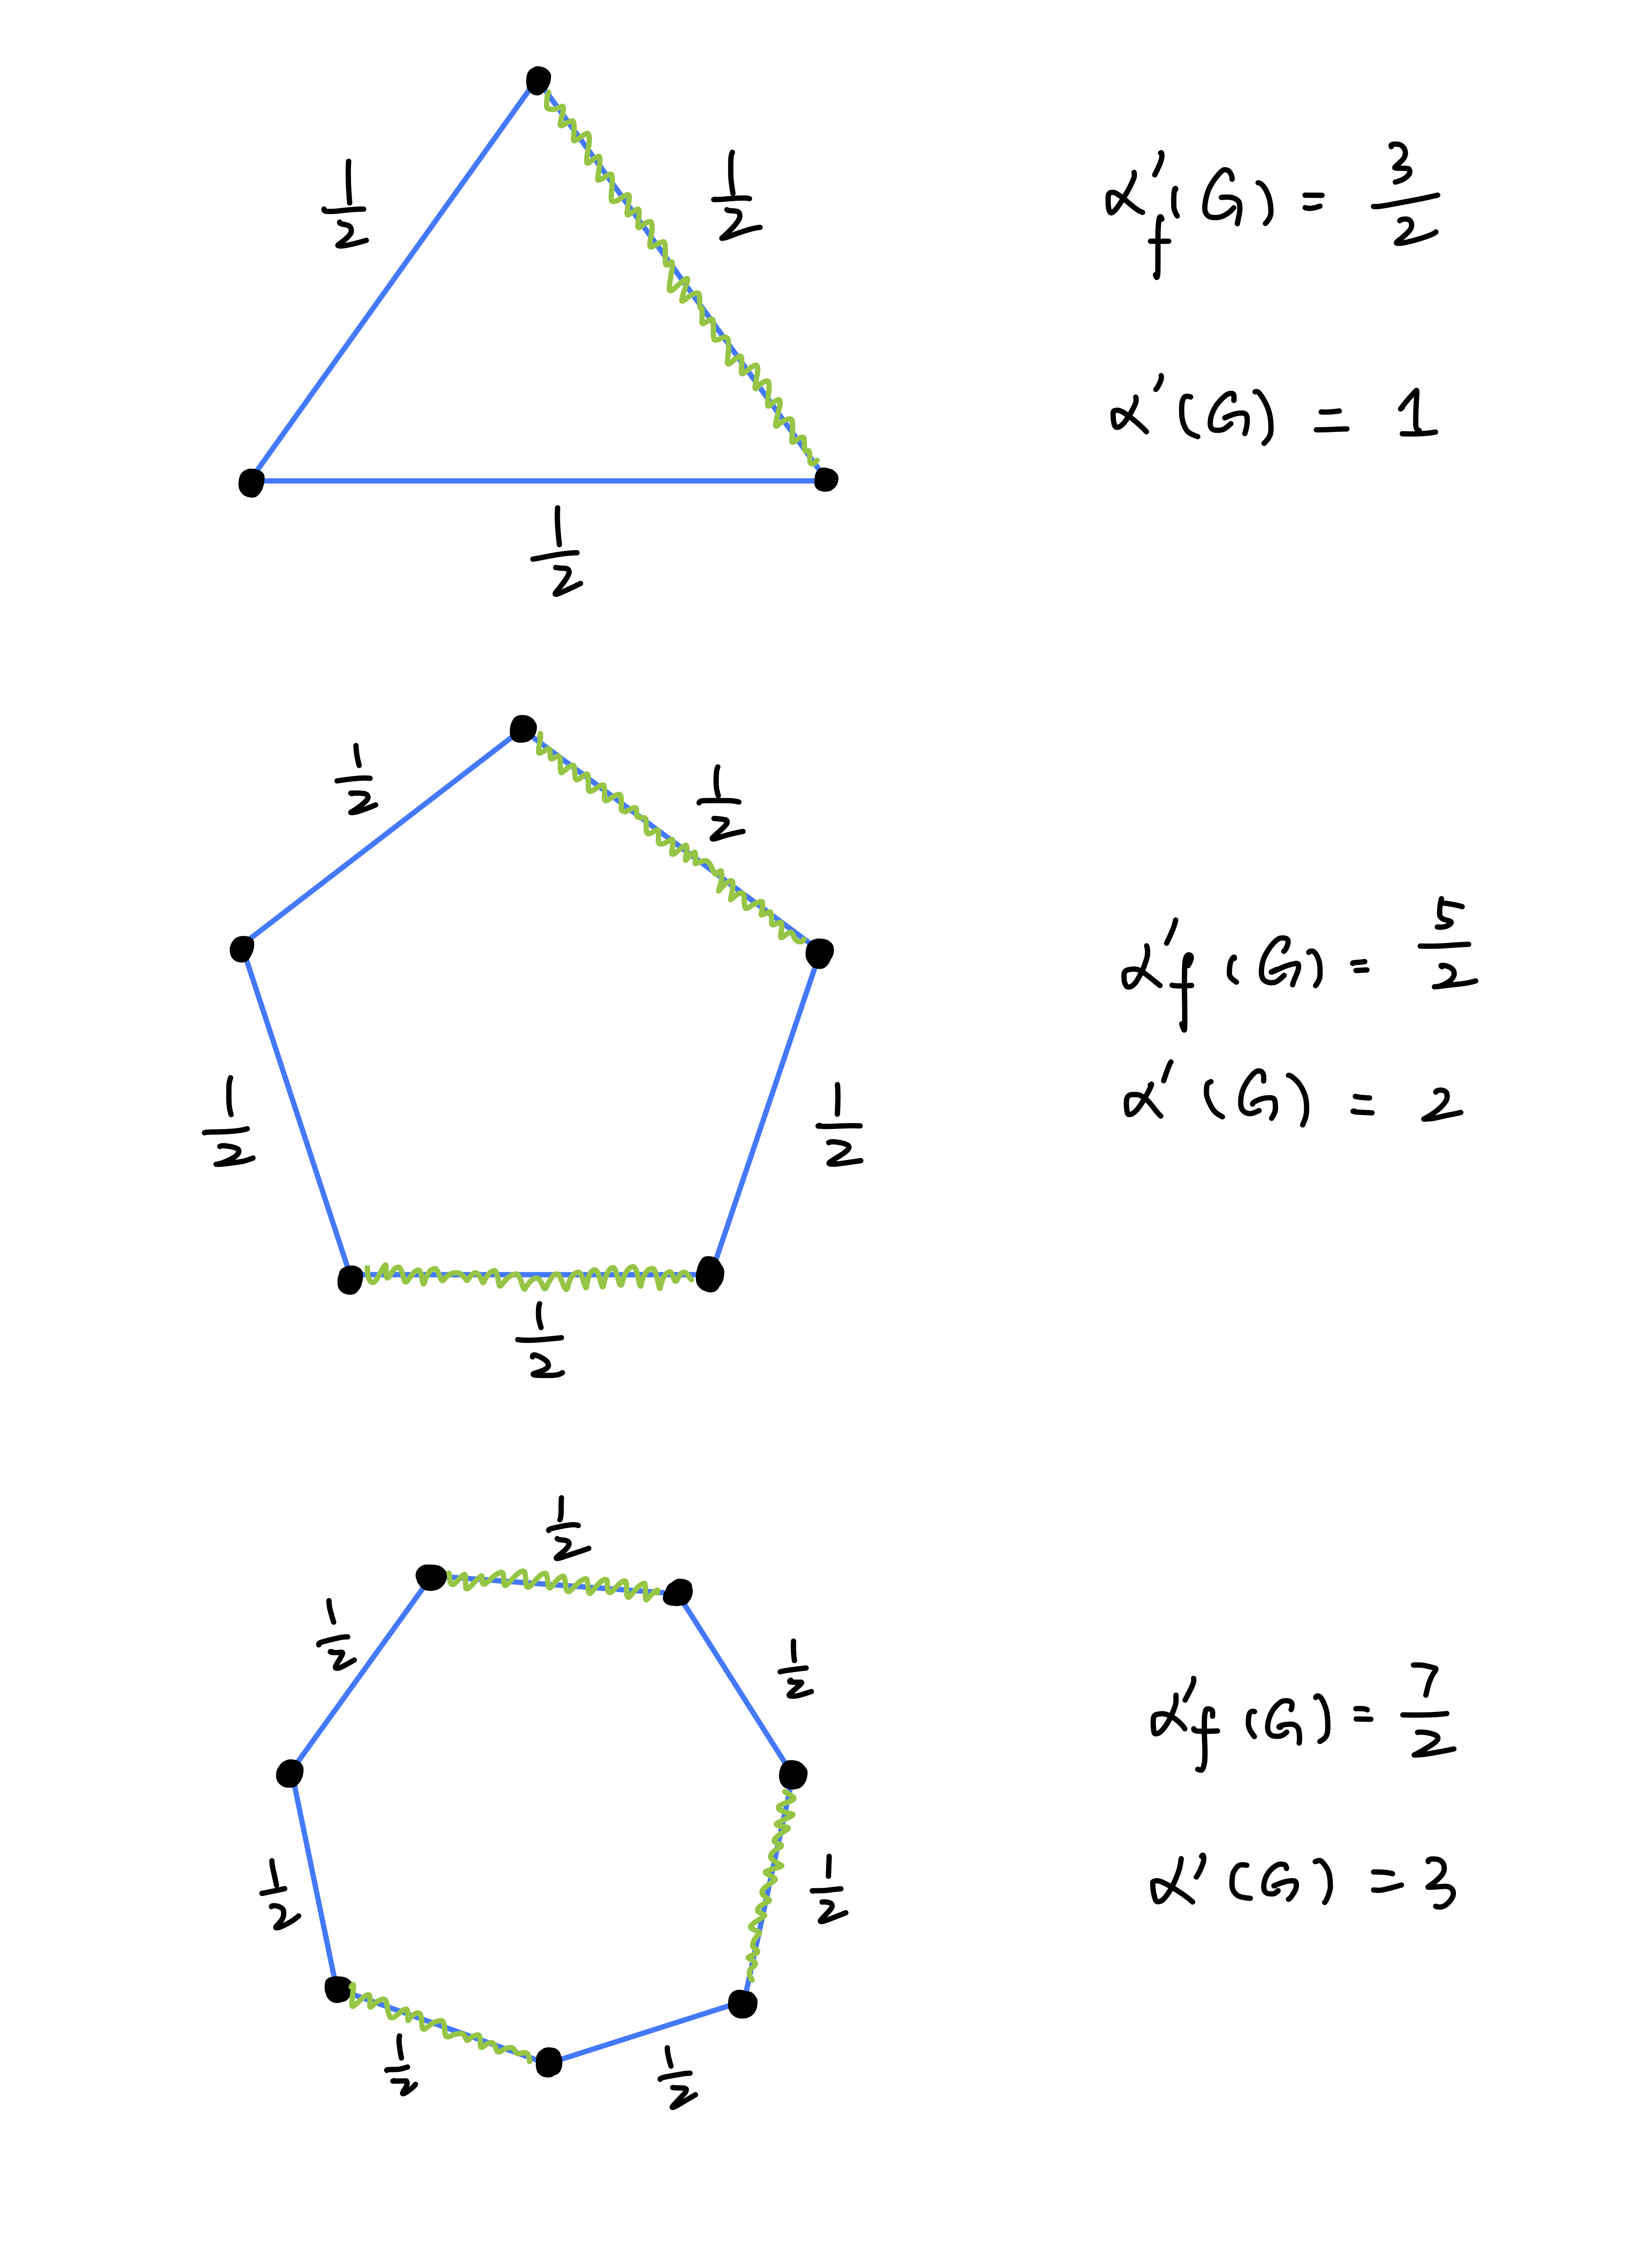
\includegraphics[scale = 0.04]{images/a.png}
        \caption{Odd cycle examples}
    \end{figure}

	Observe that as the number of edges of an odd cycle increases, the ratio $\dfrac{\alpha'_f(G)}{\alpha'(G)}$ decreases. The largest ratio $\dfrac{3}{2}$ occurs when number of edge is 3. Therefore $\alpha'_f(G) \le \dfrac{3}{2}\alpha'(G)$.

\end{document}


	
	
\end{document}